\section*{Question 3}
The develop a plan for returning the four vehicles to the four local offices, we can identify the problem as an Assignment Problem and solve the problem using the Hungarian method. As the distances are not provided between each drop-off location and office, Google Maps was used to get these distances. The shortest distance for each route was used and rounded down to be an integer. The setup of the Hungarian method and initial two steps are shown in Figure~\ref{fig:q3_initial}. After the first two steps, optimality is not reached, therefore we find an improved solution in Figure~\ref{fig:q3_answer} which we discover is an optimal solution. The optimal solution for returning the four vehicles to the four local offices is shown in Table~\ref{tab:q3}.

\begin{figure}[htp]
\centering
\caption{\label{fig:q3_initial}Hungarian Method Setup}
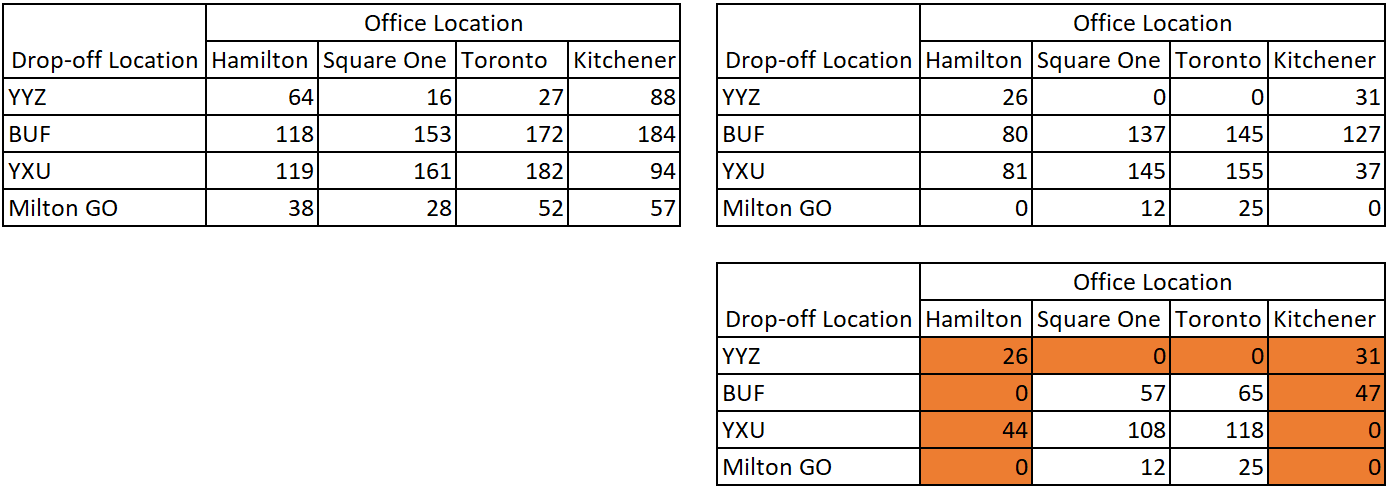
\includegraphics[width=\textwidth]{3_setup.png}
\end{figure}

\begin{figure}[htp]
\centering
\caption{\label{fig:q3_answer}Hungarian Method Optimal Solution}
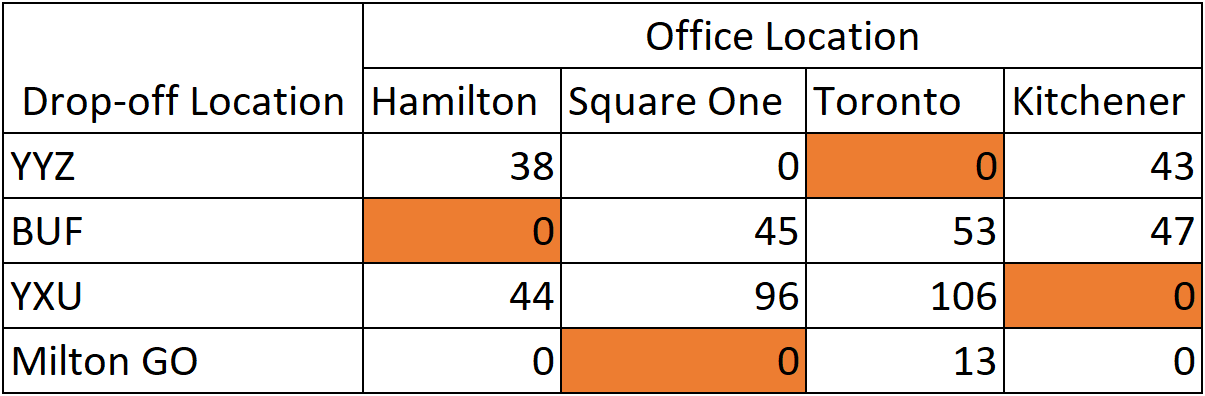
\includegraphics[width=\textwidth]{3_answer.png}
\end{figure}

\begin{table}[htp]
\centering
\caption{\label{tab:q3}Optimal Solution}
\begin{tabular}{|l|l|}
	\hline
	Drop-off Location & Return Location  \\ \hline
	YYZ               & Downtown Toronto \\ \hline
	BUF               & Hamilton         \\ \hline
	YXU               & Kitchener        \\ \hline
	Milton GO         & Square One       \\ \hline
\end{tabular}
\end{table}